\section{Fundamento teórico}

Para comenzar se deben establecer unos parámetros para con la pala, ya que lo más básico de este trabajo empieza por determinar los efectos que produce la torsión en nuestra obtención de energía.

Es por ello que se determina que la pala de la turbina eólica es un \textbf{trapecio} cuya representación simplificada la vemos en la Figura \ref{fig:pala_simp} \\\\


\textcolor{red}{\Large{CAMBIAR LA NOMENCLATURA DE LAS FIGURAS}}

\begin{figure}[H]
    \centering
    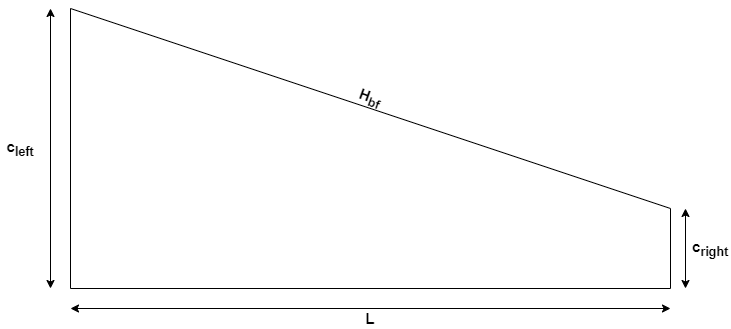
\includegraphics[width=0.7\textwidth]{images/pala simple.png}
    \caption{Representación de una pala de turbina eólica}
    \textit{Fuente: Elaboración propia}
    \label{fig:pala_simp}
\end{figure}



Lo siguiente que se debe tener presente es que se necesita también una representación de la pala de la figura \ref{fig:pala_simp} dividida en segmentos de igual largo para poder comprender el desarrollo que se realizará simulando una torsión, en la cual se girarán los segmentos un cierto ángulo los unos de los otros.

    \textbf{}
    \begin{figure}[H]
    \centering
    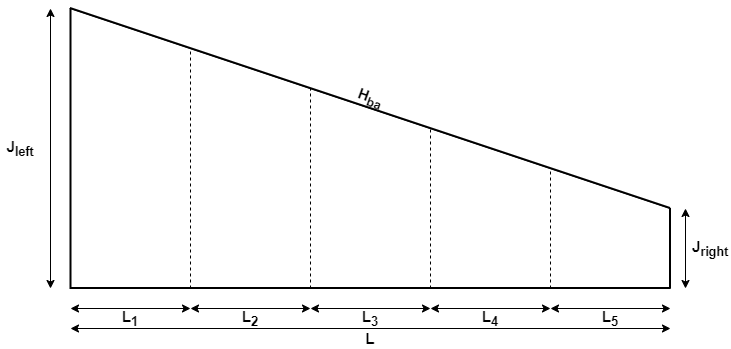
\includegraphics[width=0.7\textwidth]{images/pala simple segmentada.png}
    \caption{Representación de una pala de turbina eólica dividida en segmentos}
    \textit{Fuente: Elaboración propia}
    \label{fig:pala_dividida}
\end{figure}

Por simplicidad, la pala se dividirá únicamente en $N$ segmentos, en este caso 5. Aunque se mantenga este valor durante el trabajo y es probable que no cambie, se asociará a una variable en caso de que se quieran hacer pruebas mediante simulación en MATLAB más adelante. \\\\
    

La $L$ o \textit{longitud de pala}, vista en la Figura \ref{fig:pala_simp} es con la que se va a trabajar, por ello cada uno de los segmentos de la Figura \ref{fig:pala_dividida} tendrá el siguiente largo $\dfrac{L}{N} = \dfrac{L}{5} = L_i$  ya que se dividió $N$ número de veces. \\

Como se puede observar en la Figura \ref{fig:pala_dividida} cada segmento tiene una altura variable, esto se debe a la forma real de las palas, cuanto más cerca del buje de la turbina, mayor es el área del segmento. La altura en el centro de estos segmentos, conocida como $chord \text{ } line$ o $línea \text{ } de \text{ } cuerda$ se determinará mediante el preestablecimiento de una serie de datos y su desarrollo matemático relacionados con la pala completa.\\

Para el cálculo de la $línea \text{ } de \text{ } cuerda$ se requiere la realización de un desarrollo trigonométrico. 

\begin{figure}[H]
    \centering
    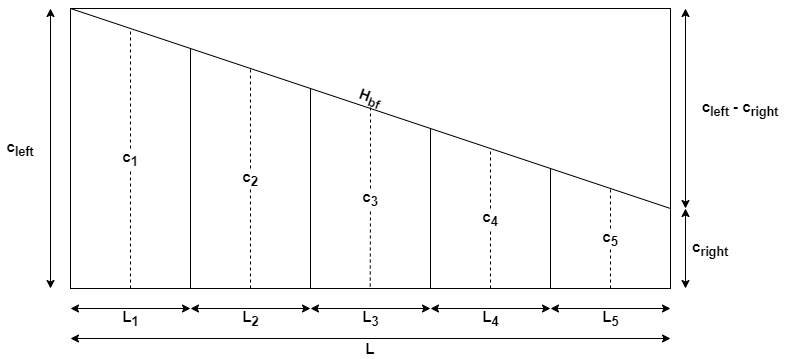
\includegraphics[width=0.9\textwidth]{images/planteo chord line.png}
    \caption{Representación parametrizada de la pala de una turbina eólica marina}
    \textit{Fuente: Elaboración propia}
    \label{fig:pala_desarrollo_chord}
\end{figure}



\begin{definicion}
En base a esta representación esquemática se puede deducir que:
$$ J_{left} = J$$
$$ J_{right} = J/D$$
$$ L_i = L/N$$
Donde,
\centering
J y D $\in \mathbb{Q+}$, \hspace{2pt} $J > D$, \hspace{2pt} $L_i$ := longitud del segmento,  $J_{left}$ := longitud simplificada del buje o hub de la pala y $J_{right}$ := longitud simplificada de la punta o tip de la pala, $i \in segmento$ y $segmento = \{1, ..., N\}$ 
\label{def_laterales_pala}
\end{definicion}


Ahora, una vez se tienen las variables básicas para conocer el resto de parámetros, se comienza con los cálculos.

\begin{definicion}
Con las variables formalizadas en la anterior definición, se define el valor $H_{bf}$ mediante el teorema de Pitágoras ya que el triángulo es rectángulo.

$$ H_{bf} = \sqrt{(J_{left} - J_{right})^{2} + L^{2}}$$
Donde,
\centering
$H_{bf}$ := borde de fuga de la pala.
\label{def_hipotenusa_pala}
\end{definicion}


A continuación, lo próximo que se debe obtener es el ángulo $\Phi$ o \textit{Ángulo de la línea del borde de arrastre de la pala de la turbina eólica}, para así conocer como decrece la $H_{bf}$ y mediante una relación trigonométrica extraída del artículo \cite{armenta2021predictive} poder obtener los valores de la \textit{Líneas de cuerda}.

\begin{figure}[H]
    \centering
    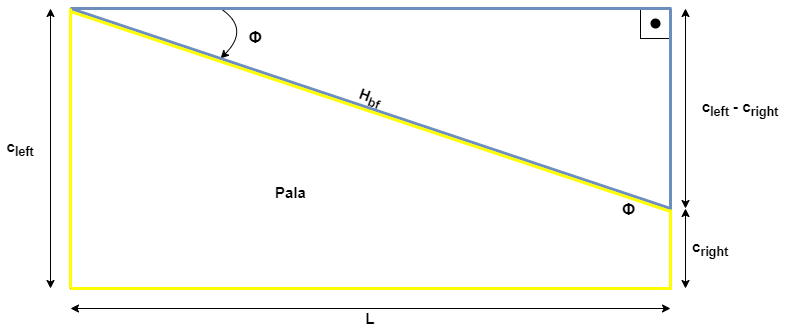
\includegraphics[width=0.9\textwidth]{images/triangulo sacar phi.drawio.png}
    \caption{Pala de la turbina en amarillo y triángulo usado para el cálculo de $\Phi$ en azul}
    \textit{Fuente: Elaboración propia}
    \label{fig:pala_calculo_phi}
\end{figure}

\begin{definicion}
En base a la figura \ref{fig:pala_calculo_phi} se puede deducir de tres formas por trigonometría el ángulo $\Phi$:
$$ \Phi = \arcsin{(\dfrac{c_{left} - c_{right}}{H_{bf}})} $$
$$ \Phi = \arccos{(\dfrac{L}{H_{bf}})} $$
$$ \Phi = \arctan{( \dfrac{\sin{(\dfrac{c_{left} - c_{right}}{H_{bf}})}}{\cos{(\dfrac{L}{H_{bf}})}} ) } $$
\label{def_angulo_phi}
\end{definicion}


El siguiente paso para calcular las $líneas \text{ } de \text{ } cuerda$ se basa en aislar trapecios mas pequeños de los que se han obtenido todos los datos menos el valor de su base menor que se tendrá que calcular, siendo este equivalente a $c$.\\

\begin{definicion}
Variables necesarias para el cálculo de las líneas de cuerda.

$$ altura_i = \dfrac{(2i - 1) \cdot L}{2N}$$
$$ diagonal_i = \dfrac{(2i - 1) \cdot H_{bf}}{2N}$$

Donde,
\centering
$altura_i$ := Longitud de la pala fragmentada para el cálculo de la línea de cuerda y $diagonal_i$ := Longitud de la hipotenusa del borde de fuga fragmentada para el cálculo de la línea de cuerda.
\label{def_variables_fragmentadas}
\end{definicion}

Por último y una vez definido todo lo necesario, se pasa al cálculo mediante el cual se obtiene el valor de todas y cada una de las $líneas \text{ } de \text{ } cuerda$ de la pala con la que se está trabajando.

\begin{definicion}
Primero se obtiene la diferencia mediante Pitágoras entre la base mayor y la menor, definida como $x_i$, después la resta de la base mayor y esta diferencia.

$$ x_i = \sqrt{diagonal_i^{2} - altura_i^{2}}$$

$$ c_i = c_{left_i} - x_i $$
\label{def_chord_line}
\end{definicion}

La siguiente figura, ilustra el ejemplo en el que para las definiciones \ref{def_variables_fragmentadas} y \ref{def_chord_line} el valor de $i$ es igual a 3. Obteniendo así $c_3$. En verde el trapecio y en magenta el triángulo del que restamos el cateto a la base mayor del trapecio.

\begin{figure}[H]
    \centering
    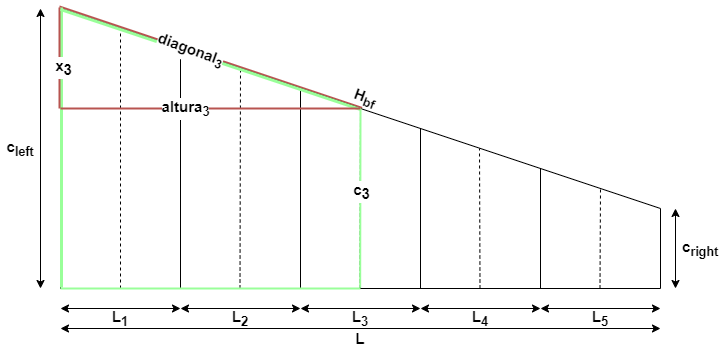
\includegraphics[width=0.9\textwidth]{images/Trapecio calculo x.png}
    \caption{Representación gráfica del cálculo realizado en las definiciones \ref{def_variables_fragmentadas} y \ref{def_chord_line}}
    \textit{Fuente: Elaboración propia}
    \label{fig:pala_calculo_phi}
\end{figure}


Una vez se ha obtenido el valor buscado $c_i$, se deberá definir todos los laterales de los segmentos de la pala, para así poder operar con ellos en pos de conseguir el área de cada uno de ellos. Esto ya fue desarrollado en el artículo \cite{armenta2021predictive}, pero en aquel caso fue usado para comprobar el error que suponía usar un rectángulo en vez de una pala simplificada. En este caso se parte directamente de la pala simplificada para evitar correcciones de errores mas adelante y porque el cálculo que se debe realizar con respecto a la obtención de energía no es tan profundo y complicado como en el artículo \cite{armenta2021predictive}. Además remarcar que para las deducciones y cálculos anteriores se bebió de este desarrollo.


\begin{definicion}
En base a esta representación esquemática y mediante relaciones trigonométricas obtuvieron:
$$ c_{left_i} = c_i + (\dfrac{L_i}{2}) \tan \varPhi$$
$$ c_{right_i} = c_i - (\dfrac{L_i}{2}) \tan \varPhi$$
\label{def:laterales_segmento}
\end{definicion}

Al igual que se deduce en el artículo \cite{armenta2021predictive}, con los datos obtenidos de los laterales de cada segmento, se puede trabajar con una forma de trapecio y encontrar el área de los segmentos que se definieron en la Figura \ref{fig:pala_dividida}.\\

Aparte, con esta definición se ve que en la Figura \ref{fig:pala_desarrollo_chord} los valores de $c_{left_i}$ y de $c_{right_i}$ que se observan, realmente serían equivalentes a $c_{left_1}$ y a $c_{right_5}$, respectivamente. Estos son definidos a priori debido a su importancia para caracterizar la pala de manera correcta y con las dimensiones que el usuario desee.

\begin{definicion}
Se determina el área de los segmentos:
$$ S_{i} = \dfrac{(c_{left_i} + c_{right_i})}{2N} \cdot L_i $$
Donde,
\centering $S_i$ := Área del segmento.
\label{def:area_segmentos}
\end{definicion}


A continuación, se supone que los segmentos están ensartados por una línea imaginaria que ayudará al estudio de la torsión mediante giros de los segmentos alrededor suya. \\

Esta línea imaginaria pasará por el centro de masas de todos los segmentos. Delineando rectas desde cada esquina a la contraria,genera un punto en el centro de la figura, en el que se cortan, siendo este el centro de masas. También se puede, observando la Figura \ref{fig:pala_dividida} hallar el punto central tanto de la recta del buje como de la de la punta y trazar una recta de uno a otro, esta recta también pasa por el centro de masas de cada uno de los segmentos.\\

Cuando se ha obtenido esta recta imaginaria, se puede pasar a determinar lo que conocemos como $brazo$. Cada medida de brazo va desde el punto central del buje siguiendo la recta que se trazó hasta la $línea \text{ } de \text{ } cuerda$ del segmento.


    \begin{figure}[H]
    \centering
    \includegraphics[width=1\textwidth]{images/explicación brazo.png}
    \caption{Representación gráfica del brazo de la pala}
    \label{fig:exp_brazo}
    \textit{Fuente: Elaboración propia}
\end{figure}

\begin{definicion}
El brazo viene definido de la misma manera que se halló la hipotenusa del borde de fuga, solo que en este caso la resta es de las mitades de los lados de la pala. Una vez se tiene la recta que pasa por los centros de masa se determina el valor de cada uno de los brazos.
$$ cateto \text{ } buje = \dfrac{J_{left}}{2} - \dfrac{J_{right}}{2} $$

$$ R \text{ } brazo = \sqrt{cateto \text{ } buje^{2} + L^{2}}$$

$$ brazo_i = \dfrac{(2i -1) \cdot R \text{ } brazo}{2N} $$
Donde, $cateto \text{ } buje$ := Medida de buje o $J_{left}$ reducida para su utilización en la obtención del brazo, $R brazo$ := Recta completa del brazo antes de dividirla dependiendo del segmento y \hspace{10pt} $brazo_i$ := Distancia entre el centro de $J_{Left}$ y el centro de masas del segmento correspondiente.
\centering 
\label{def:brazo}
\end{definicion}

\subsection{Estudio del torque sin ángulo de cabeceo}
\label{section:torque_pala_horizontal}

%Minuto 30 de la parte 1
\textcolor{red}{Va a haber giro porque la pala por la parte de arriba está mas redondeada por la parte de arriba que por la de abajo, entonces por Bernouilli tienes mas recorrido por arriba  que por abajo, lo que obliga que la velocidad por arriba sea mayor por tanto la presión sea menor, haciendo que tengamos un gradiente de presión y por ello una fuerza de sustentación. Simplemente porque la pala no es simétrica. Esta no es la situación mas favorable, la más favorable es la de la siguiente sección. \\\\
{\Large DEFINIR CON PALABRAS DECENTES, ES LITERALMENTE LA TRANSCRIPCIÓN QUE DIJO}}





















\subsection{Estudio del torque con ángulo de cabeceo}
\label{section:torque_giro_inicial}

Se han presentado algunos de los conceptos básicos, ahora se introduce el ángulo $ \theta_1 $, que es la constante definida como el \textit{ángulo de cabeceo} que sufrirán todos y cada uno de los segmentos que son paralelos al plano horizontal, desde el cual se presenta el viento que incidirá en nuestra pala.\\


En esta primera sección se estudiará qué ocurre en término de fuerzas, torque y momento cuando se gira toda nuestra pala únicamente el ángulo de cabeceo $ \theta_1 $. \\


Es cierto que se podría no girar la pala este ángulo $ \theta_1 $, pero por comodidad de cálculo y para establecer un ángulo de ataque del viento paralelo a la horizontal se realizará de esta manera.\\


Al haber inclinado todos los segmentos un ángulo $ \theta_1 $ se genera la situación en la que el viento incide en el centro del segmento con el mismo ángulo con el que se inclina la pala. \\

    \textbf{}
    \begin{figure}[H]
    \centering
    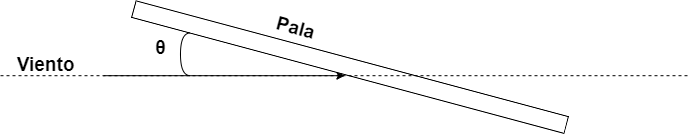
\includegraphics[width=0.8\textwidth]{images/dibujo angulo ataque.drawio.png}
    \caption{Ángulo de ataque del viento con respecto a la pala}
    \textit{Fuente: Elaboración propia}
    \label{fig:dibujo_angulo_ataque}
\end{figure}

La fuerza del viento que incide en la pala se puede descomponer en 2, la tangencial y la normal. \\

    \textbf{}
    \begin{figure}[H]
    \centering
    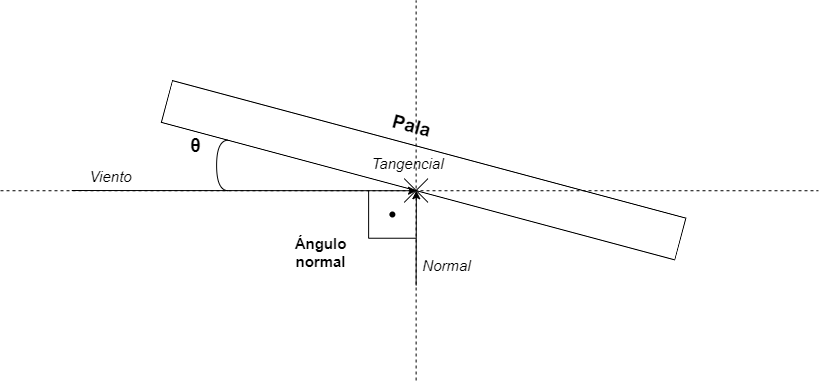
\includegraphics[width=1\textwidth]{images/dibujo fuerzas.drawio.png}
    \caption{Descomposición de vectores de fuerzas}
    \textit{Fuente: Elaboración propia}
    \label{fig:dibujo_fuerzas}
\end{figure}


Como se puede ver en la figura \ref{fig:dibujo_fuerzas} el vector fuerza normal es perpendicular al ángulo de ataque del viento, mientras que el vector fuerza tangencial recorre de manera paralela la línea central de la pala.

%  \begin{definicion}
%  La fuerza normal genera un ángulo definido por:
%  $$ n = \dfrac{\pi}{2} - \theta_1 $$
%  Donde,
%  \centering $n$ := ángulo normal.
%  \end{definicion}

 \begin{definicion}
 La fuerza normal viene definida por la siguiente expresión:
  $$ f \text{ } normal_i = F \text{ } viento_i \cdot \sin{\theta_1}$$
Donde,
\centering $F \text{ } viento$ := Fuerza generada por el viento en cada segmento de la pala y $f \text{ } normal$ := Fuerza perpendicular al viento, generada por el choque de este con la pala de la turbina eólica.
 \label{def:fuerza_normal}
 \end{definicion}
 
  La componente paralela a la pala, que se ha definido como tangencial se obviará debido a que no genera momento de torsión o torque. 
  
  \begin{definicion}
El momento de giro o torque se define como:
 $$ torque_0 = f normal_i \times brazo$$
Donde,
\centering $torque_0$ := Momento de fuerza de giro solo con ángulo de cabeceo.
  \label{def:torque_inicial}
 \end{definicion}
 

 En la Definición \ref{def:torque_inicial} se encuentra un producto vectorial entre la $fuerza  \text{ }perpendicular \text{ } o \text{ } normal$ y el $brazo$. Pero estas dos variables son perpendiculares la una a la otra. Esto se puede ver ya que $brazo$ es completamente paralelo a la $fuerza \text{ } tangencial$. Esto demuestra la perpendicularidad y hace que la Definición \ref{def:torque_inicial} que contenía un producto vectorial de dos parámetros perpendiculares sea definitivamente un producto algebraico, dando lugar a:
 
 
  \begin{definicion}
  El torque termina siendo un producto algebraico.
 $$ torque_0_{i} = f \text{ } normal_i \cdot brazo_i$$
 \label{def:torque_algebraico_inicial}
 \end{definicion}
 
 
 \begin{definicion}
 La suma de los torques con un ángulo de cabeceo se conoce como torque global.
 $$ torque \text{ } global_0 \text{ } = \sum_{i=1}^{N} torque_0_{i} $$
\label{def:torque_global}
\end{definicion}
 
 \\\\Ahora se introduce otro concepto, se trata de la \textit{fuerza del viento}. Gracias a este parámetro, se podrá conocer la fuerza normal que se está produciendo en toda la pala mediante la definición \ref{def:fuerza_normal}.
 
 
 \begin{definicion}
 La fuerza del viento para la pala viene dada por:
 
 $$ F \text{ } viento_i = \dfrac{1}{2} \text{ } \rho \cdot S_i \cdot u^2$$
Donde,
 \centering  $\rho = 1.225 \text{ } \dfrac{Kg}{m^3}$ y $u$ := velocidad del viento.
 \label{def:fuerza_viento_inicial}
 \end{definicion}
 
\vspace{15pt} Entendido esto, ya se podría pasar a calcular el valor del $torque \text{ } global_i$.
 
 
 
 
 
 
 
 
 
 
 
 
 \subsection{Estudio del torque con ángulo de cabeceo y torsión de la pala}
\label{section:torque_giro_torsion}

La única diferencia entre este apartado y el anterior es el ángulo de giro de los segmentos. En la sección \ref{section:torque_giro_inicial} se vió como todos los segmentos giraban únicamente un determinado \textit{ángulo de cabeceo}, pero ahora y en pos del estudio de la torsión, el ángulo que se girarán vendrá dado por la siguiente definición: 


\begin{definicion}
Dados el ángulo inicial de giro $\theta_1 $ y una variación de giro constante (o no) $\Delta_\theta$ se define el ángulo de torsión de cada segmento como:
$$\theta_i = \theta_{i-1} + \Delta_\theta$$ 
Donde,
\centering $i \in segmento \wedge (i > 1)$

\label{def:theta_cte}
\end{definicion}


\begin{definicion}
Como se menciona, la variación $\Delta_\theta$ puede que no sea constante por conveniencia a la hora de calcular resultados futuros, por ello la definición también puede darse de la siguiente forma:
$$\theta_i = \theta_{i-1} + \Delta_{\theta_{i}}$$ 
Donde,
\centering $i \in segmento \wedge (i > 1)$
\label{def:theta_nocte}
\end{definicion}


Esto provoca que algunas de las definiciones anteriores se vean alteradas por el cambio que presenta la variable $\theta_i$.\\

% \begin{definicion}
%  La fuerza normal genera un ángulo de:
%  $$ n_i = \dfrac{\pi}{2} - \theta_i $$
 
%  Donde,
%  \centering $i \in segmento$
%  \end{definicion}

 \begin{definicion}
  Su fuerza se define como:
  $$ f \text{ } normal_i = F \text{ } viento_i \cdot \sin{\theta_i}$$
  \label{def:fuerza_normal_torsion}
 \end{definicion}

El resto de fórmulas no varían debido a que no dependen del ángulo $\theta_i$, tienen exactamente la misma definición. Pero en el caso del \textit{torque global} si que cambia, ya que la suma de torques nos aportará un conjunto de valores diferentes y que servirán como estudio. \\\\


{\Large TERMINAR DE DEFINIRLO}
  \begin{definicion}
  El torque termina siendo un producto algebraico.
 $$ torque_0_{i} = f \text{ } normal_i \cdot brazo_i \cdot \sin{\Delta_{\theta_{i}}}$$
 Donde,
 \centering $\sin{\Delta_{\theta_{i}}}$ := 
 \label{def:torque_algebraico_torsion}
 \end{definicion}
 

\begin{definicion}
 La suma de los torques con un giro inicial se conoce como torque global.
 $$ torque \text{ } global_1 \text{ } = \sum_{i=1}^{N} torque_1_{i} $$
Donde,
\centering $torque \text{ } global_1$ := Suma de torque de los N segmentos.
 \label{def:torque_global_1}
\end{definicion}






















\subsubsection{Cálculo de la potencia del sistema}
 
 Una vez se tiene todo lo necesario para el cálculo del torque, se puede pasar al siguiente escalón que sería la potencia. Esta es una unidad de medida que permitirá conocer si el estudio que se está realizando está siendo fructífero, cuanta mayor cantidad de energía se genere, mejor.
 
  \begin{definicion}
 La potencia del sistema con un ángulo de caebceo se define como:
 $$ potencia_0 = torque \text{ } global_0 \cdot \Omega $$ 
 
 Donde,
  \centering $\Omega$ := velocidad de giro o angular de la pala y $potencia_0$ := Energía del sistema unicamente con un cierto ángulo de cabeceo.
 \label{def:potencia_giro_inicial}
 \end{definicion}
 
   \begin{definicion}
 La potencia del sistema con un giro inicial y torsión se define como:
 $$ potencia_1 = torque \text{ } global_1 \cdot \Omega $$ 
 
 Donde,
 \centering $potencia_1$ := Energía del sistema con un cierto ángulo de cabeceo y segmentos torsionados.
 \label{def:potencia_giro_segmentos}
 \end{definicion}
 
 
 \textcolor{red}{La potencia está en W (Watts) o J/s (Julio/segundo) porque el torque está en N/m (Newton/metro) o J y $\Omega$ es en 1/s o $s^-1$} \\

 
 Como se puede observar, se calculó dos veces la potencia, una por cada apartado estudiado. La definición \ref{def:potencia_giro_inicial} corresponde a la sección \ref{section:torque_giro_inicial} que se referencia con un $0$ ya que es la situación inicial y más básica. Mientras que la definición \ref{def:potencia_giro_segmentos} corresponde a la sección \ref{section:torque_giro_torsion} que se ha referenciado con un $1$ ya que nace de la primera.
 
 
 
\subsubsection{EXPLICACIÓN DE LA VELOCIDAD ANGULAR}
 
 
\textcolor{red}{\Large{MEJORES MATERIALES: FIBRA DE VIDRIO REFORZADA CON PLÁSTICO (1.50–2.10) O FIBRA DE CARBONO REFORZADA CON PLÁSTICO( g/cm3	1.8–2.0) y rho = 1700 $kg/m^3$ (Fibra de vidrio-epoxi) }}
 
 
 \subsection{Rendimiento de las potencias}
 \label{section:rendimiento}
 
Realizada la definición de cada una de las fórmulas necesarias para el cálculo de la potencia, se pasa a la comparación de estas. La comparación de potencias nos da como resultado un rendimiento, con este seremos capaces de dictaminar si la torsión de la pala genera una variación en la potencia obtenida.
 
   \begin{definicion}
El rendimiento del sistema viene definido por:
 $$ \eta = \dfrac{potencia_1}{potencia_0} $$ 
 
 Donde,
  \centering $\eta$ := eficiencia respecto a la energía obtenida en dos casos estudiados.
 \label{def:rendimiento_potencias}
 \end{definicion}
 
 Una vez se ha definido el rendimiento y se calcula en base a los resultados obtenidos mediante asignación de valores a variables estándar y aplicando estos a las definiciones relacionadas, se pueden dar 3 escenarios:
 

\begin{enumerate}
    \item $\eta < 1$
        \begin{itemize}
            \item En caso de obtener un valor por debajo de 1, quiere decir que la torsión que se aplicó en el caso estudiado, ha reducido la obtención de energía con respecto al caso base. 
        \end{itemize}
    \item $\eta ~= 1$
        \begin{itemize}
            \item Si el valor obtenido es muy próximo a 1, entonces el caso base y el estudiado proporcionan valores similares de obtención de energía.
        \end{itemize}
    \item $\eta > 1$
        \begin{itemize}
            \item Este es el valor buscado y el objetivo del estudio, que una pala con torsión obtenga más energía que una sin ello.
        \end{itemize}
\end{enumerate}

Cabe recalcar que se deberán hacer numerosas pruebas con diferentes configuraciones de valores .... (SEGUIR)
 
\subsection{Primeras pruebas en MATLAB}

Desarrollado todo el fundamento teórico detrás del estudio que se está realizando y con el que se está tratando de conocer si mediante torsión de las palas de una turbina eólica se obtiene más energía, menos o la misma que si no se torsionasen, se debe avanzar y comenzar a hacer cálculos empíricos. \\

Estos cálculos y representaciones se realizarán mediante MATLAB, de la manera más ordenada y arbitraria posible. Con esto se busca la manera más simple de poder modificar las variables más sencillas que envuelven a los cálculos, para así poder cambiarlas a placer. \\

Algunas variables como, $L$ y $\Theta_1$ deben ser establecidas por el propio estudiante, dando así un mayor juego a la amplitud de resultados posibles. \\
